\documentclass{../cssheet}

%--------------------------------------------------------------------------------------------------------------
% Basic meta data
%--------------------------------------------------------------------------------------------------------------

\title{Darstellende Geometrie}
\author{Prof. Dr. Christian Spannagel}
\date{\today}
\hypersetup{%
    pdfauthor={\theauthor},%
    pdftitle={\thetitle},%
    pdfsubject={Aufgabenblatt Geometrie},%
    pdfkeywords={geometrie}
}


%--------------------------------------------------------------------------------------------------------------
% document
%--------------------------------------------------------------------------------------------------------------

\begin{document}
\printtitle

In diesem Aufgabenblatt sollt ihr verschiedene Körper in Dreitafelprojektion, in Frontschau und in Vogelschau zeichnen. Überlegt euch jeweils immer, welche Teile der Körper in wahrer Größe abgebildet werden.


\textbf{Aufgabe 1 (Warmlaufen):}  Zeichnet folgende Körper in Dreitafelprojektion. 
\begin{enumerate}[a)]
\item eine Dreieckssäule
\item eine Sechsecksäule
\end{enumerate}

\textbf{Aufgabe 2 (Quadratische Pyramide):}  Betrachtet eine regelmäßige quadratische Pyramide mit Kantenlänge $a=\SI{10}{\cm}$.
\begin{enumerate}[a)]
\item Zeichnet sie mit zwei unterschiedlichen Grundrissen in Dreitafelprojektion wie hier angegeben.
\begin{center}
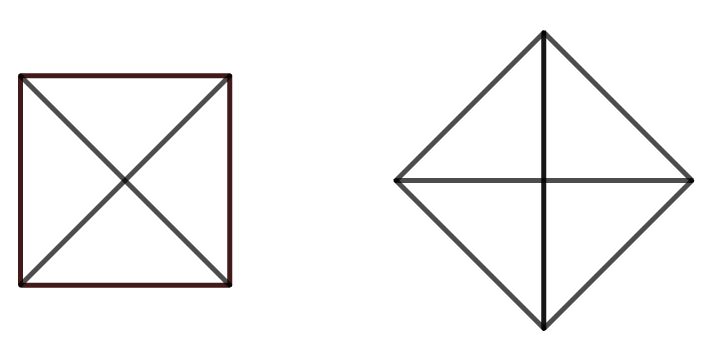
\includegraphics[width=6 cm]{quad-pyramide.png}
\end{center}
\item Zeichnet für beide Lagen die Frontschau und die Vogelschau der Pyramide. 
\end{enumerate}

\textbf{Aufgabe 3 (Tetraeder):}  Betrachtet eine regelmäßige Dreieckspyramide mit Kantenlänge $a=\SI{10}{\cm}$.
\begin{enumerate}[a)]
\item Zeichnet sie mit zwei unterschiedlichen Grundrissen in Dreitafelprojektion wie hier angegeben.
\begin{center}
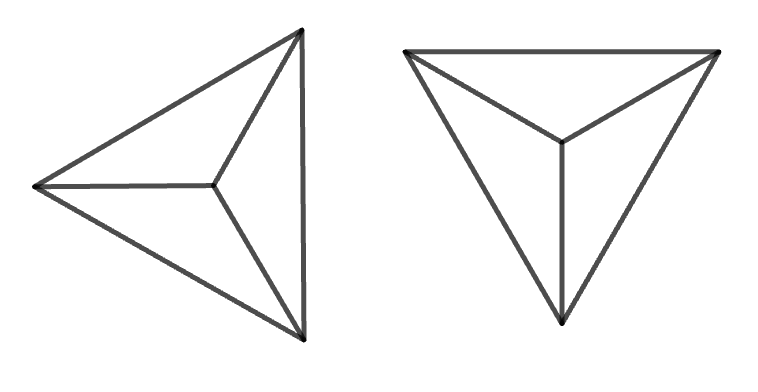
\includegraphics[width=6 cm]{tetraeder.png}
\end{center}
\item Zeichnet auch hier wieder für beide Lagen die Frontschau und die Vogelschau der Pyramide. 

\end{enumerate}

Die Aufgaben orientieren sich an: Krauter, S. \& Bescherer, C. (2013). \emph{Erlebnis Elementargeometrie} (2. Aufl.). Berlin, Heidelberg: Springer.

\printlicense

\printsocials
\end{document}
